%
% Draft  document waterfox.tex
%
 
\documentclass{article}  % Latex2e
\usepackage{graphicx,lscape,subfigure}
 

\title{Install the Waterfox Web Browser on a Linux system}
\author{Neville Jackson}
\date{23 Apr 2022} 

\begin{document} 

\maketitle      

\section{Introduction} 
The Waterfox Web Browser is a fork of Mozilla. It is similar to Firefox, but is independently maintained. It is currently owned by {\em System1} which is a research organisation involved in software development for statistical applications using R . 

Waterfox is not currently available for download in any of the Linux distros which I use (Debian, Void, Solus). I decided to install it in Void Linux. The following is an account of my install procedure

\section{Obtain the download file}
Go to the waterfox website~\cite{wate:22}
\begin{verbatim}
https://www.waterfox.net/download
\end{verbatim}
Download the file
\begin{verbatim}
 waterfox-G4.1.1.1.en-US.linux-x86_64.tar.bz2
\end{verbatim}

\section{Unpack the download file}
Move the download file away from the Download directory to somewhere sensible where you can unpack it. Dont put it anywhere in {\em /usr} because that is reserved for software controlled by the package system. Options are 
\begin{itemize}
\item in {\em /usr/local/...} 
\item in your home directory
\end{itemize}
I choose {\em /usr/local}  so I made a directory {\em /usr/local/src} and copied the .bz2 file there.

That download file is a tar archive compresses with the {\em bzip2} program. To unpack it  got to the {\em /usr/local/src} directory and do 
\begin{verbatim}
bzip2 -dc waterfox-G4.1.1.1.en-US.linux-x86_64.tar.bz2 | tar xvf -
\end{verbatim}
it will make a directory called {\em waterfox} which will contain all the unpacked material as follows
\begin{verbatim}
[nevj@trinity waterfox]$ ls
application.ini     libmozavcodec.so  libnssutil3.so  plugin-container
browser             libmozavutil.so   libplc4.so      precomplete
defaults            libmozgtk.so      libplds4.so     removed-files
dependentlibs.list  libmozsandbox.so  libsmime3.so    update-settings.ini
fonts               libmozsqlite3.so  libsoftokn3.so  updater
gmp-clearkey        libmozwayland.so  libssl3.so      updater.ini
icons               libnspr4.so       libxul.so       waterfox
libfreeblpriv3.so   libnss3.so        omni.ja         waterfox-bin
liblgpllibs.so      libnssckbi.so     platform.ini
\end{verbatim}

\section{How to install this unpacked material?}
We have to decide what all these files are for? Well, firstly, that file called {\em waterfox} looks like a binary, so lets check
\begin{verbatim}
[nevj@trinity waterfox]$ file waterfox
waterfox: ELF 64-bit LSB pie executable, x86-64, version 1 (SYSV),
 dynamically linked, interpreter /lib64/ld-linux-x86-64.so.2,
 BuildID[sha1]=1473cfde0d27954992968743ce38e3661efb0cd3,
 for GNU/Linux 3.2.0, stripped
\end{verbatim}
Yes, that is an executable file. So what is {\em  waterfox-bin}?  A quick check with {\em cmp} reveals it is just an exact copy of {\em waterfox}.  No idea why?

So before we install it, how about we check if it will run? Just type {\em ./waterfox}, and yes it runs and brings up a browser window, but nothing appears in the applications menu, and there is no desktop icon.  A proper install might fix that. 

We need to put the binary in some {\em bin} directory, but not {\em /bin} and not {\em /usr/bin}. So I opt for {\em /usr/local/bin}
\begin{verbatim}
ln /usr/local/src/waterfox/waterfox /usr/local/bin/waterfox
\end{verbatim}
That is all, I use a link rather than copying the executable file to /usr/local/bin because when waterfox executes it sets its paths relative to the location of the executable file.  Now I do not have to be in {\em /usr/local/src/waterfox} to execute it, I can just type {\em waterfox} from anywhere, because {\em /usr/local/bin} is in my {\em PATH}. 

\subsection{Getting an app menu item and an icon}
There is still a lot of material in {\em /usr/local/src/waterfox} and we need to put it somewhere where the system can find it. The same material for firefox is in {\em /usr/lib/firefox} on my system, so I opt for {\em /usr/local/lib/waterfox}. So copy it over
\begin{verbatim}
cd /usr/local/src/waterfox
mkdir /usr/local/lib/waterfox
cp -r * /usr/local/lib/waterfox
cd /usr/lib
ln -s /usr/local/lib/waterfox waterfox
\end{verbatim}
Now I magically get an entry for Waterfox Web Browser in the Applications Menu, but still no desktop icon. Why the link?  Well  my system only seems to look in {\em /usr/lib} when it is looking for applications. Without the link, I dont get an entry in the Applications Menu.

Now for the icon. My system defines material for desktop icons in {\em /usr/share/applications}.
\begin{verbatim}
/usr/share/applications
[nevj@trinity applications]$ ls
firefox.desktop                     
gcr-prompter.desktop              
gcr-viewer.desktop               
gtk3-icon-browser.desktop       
........
mimeinfo.cache
uxterm.desktop
xscreensaver-properties.desktop
xterm.desktop
\end{verbatim}
 We need to look at the {\em firefox.desktop} file and modify it to make a {\em waterfox.desktop} file . Fortunately someone has already done that , and I was able to get the following from the waterfox website
\begin{verbatim}
[Desktop Entry]
Version=1.0
Name=Waterfox Web Browser
Comment=Browse the World Wide Web
GenericName=Web Browser
Keywords=Internet;WWW;Browser;Web;Explorer
Exec=waterfox %u
Terminal=false
X-MultipleArgs=false
Type=Application
Icon=waterfox
Categories=GNOME;GTK;Network;WebBrowser;
MimeType=text/html;text/xml;application/xhtml+xml;application/xml;application/rss+xml;application/rdf+xml;image/gif;image/jpeg;image/png;x-scheme-handler/http;x-scheme-handler/https;x-scheme-handler/ftp;x-scheme-handler/chrome;video/webm;application/x-xpinstall;
StartupNotify=true
Actions=new-window;new-private-window;

[Desktop Action new-window]
Name=Open a New Window
Exec=waterfox -new-window

[Desktop Action new-private-window]
Name=Open a New Private Window
Exec=waterfox -private-window
\end{verbatim}
 Now where do we put it?
We take our clue again from firefox. The file {\em firefox.desktop} is in {\em /usr/share/applications}. We cant put {\em waterfox.desktop} there, beacuse that is inside the package system, so we need to put it in {\em /usr/local/share}, so
\begin{verbatim}
cd /usr/local/share
mkdir applications
cd /usr/local/src/waterfox
cp waterfox.desktop /usr/local/share/applications
cd /usr/share/applications
ln -s /usr/local/share/applications/waterfox.desktop waterfox.desktop
\end{verbatim}
Again the link is necessary to get the system to detect the presence of {\em waterfox.desktop} file
The icon now appears on the display background. 
Install succedssful. 

\section{Testing}
The browser starts from either the icon or the App Menu. It looks similar to {\em firefox}. I can put in some web addresses and start browsing. An image of the browser window is showewn in Figure~\ref{fig:waterfox}
%\documentclass{article}
%\usepackage{graphicx,subfigure}
%\begin{document}

\begin{figure}[!h]
  \centering
   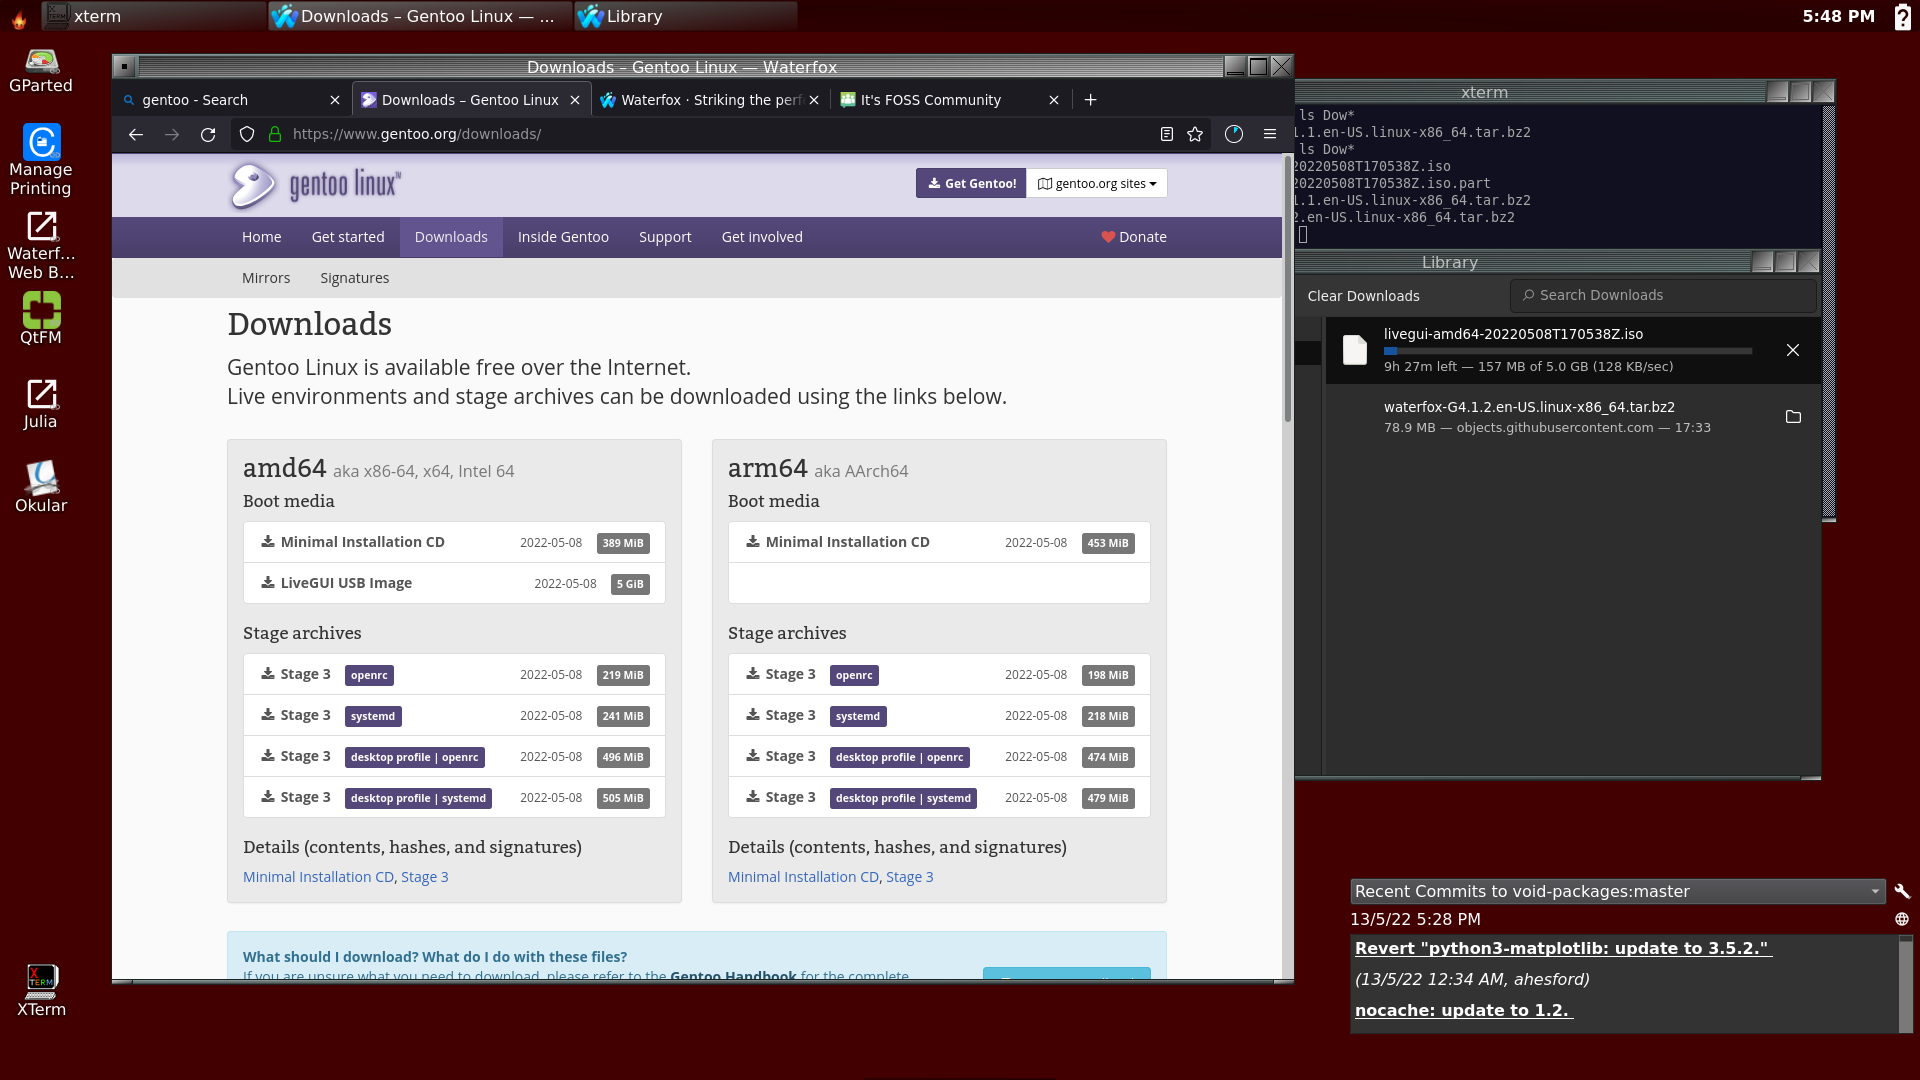
\includegraphics[totalheight=3.2in,width=1.0\textwidth]{watlum.png}
  \caption{Screenshot of Waterfox browser window running in Lumina Desktop}
  \label{fig:waterfox}
\end{figure}

%\end{document}


It puts coloured tabs on the screen for frequently accessed sites, and there is a dropdown menu on the top right for configuration. 


\subsection{Acknowledgment}

\begin{thebibliography}{99}

\bibitem{wate:22} 
Waterfox website. URL https://www.waterfox.net

\end{thebibliography}
\end{document}
